\chapter{OPERATIONAL FORECASTING FOR UTILITIES}
\label{chap:operations}

We produce operational forecasts for each utility scale solar power
plant and an estimate of the distributed generation for Arizona Public
Service (APS), Public Service Company of New Mexico (PNM), and Tucson
Electric Power (TEP).
A rough map of the balancing areas that each utility is responsible
for and the locations of their power plants is shown in
\cref{fig:utilitymap}.
At the time of this writing, utilities are primarily concerned with
day ahead and hour ahead solar power forecasts to help schedule or
trade power.
The production of operational solar power forecasts for electric
utilities informs how we judge forecast quality, the types of
forecasts we study, and it ensures the products of our research are
used.

\begin{figure}[htb]
\centering
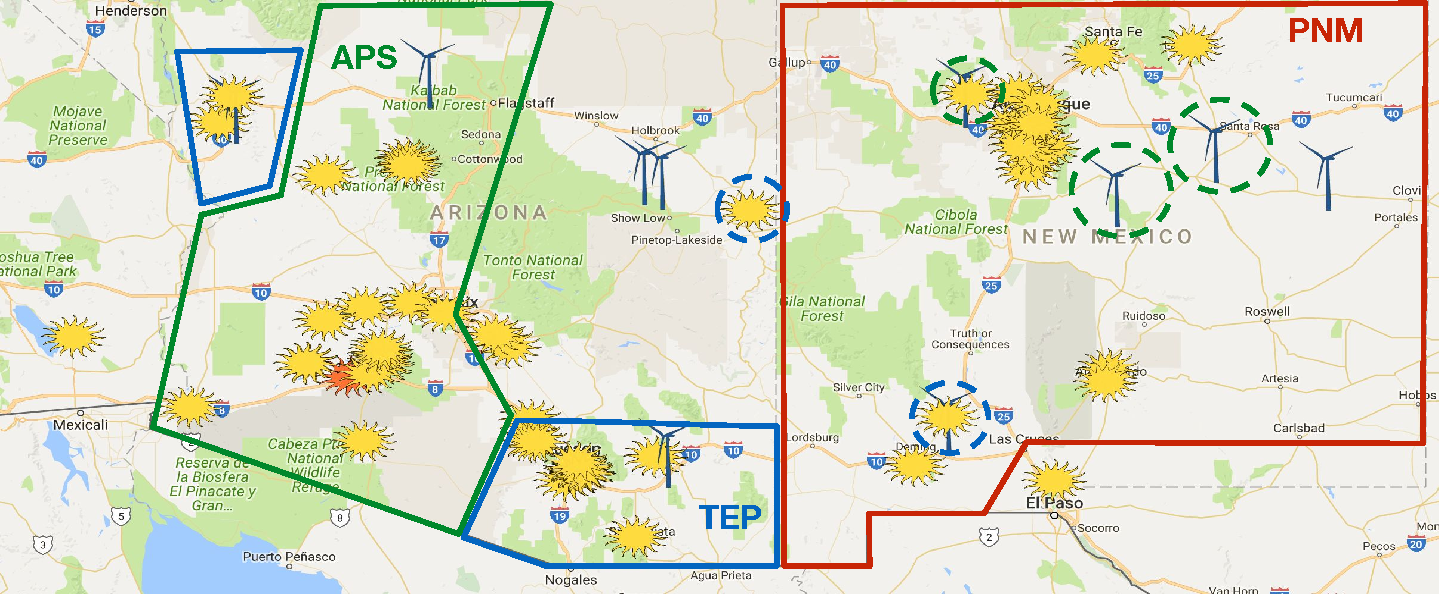
\includegraphics[width=0.9\textwidth]{figs/fxmap.pdf}
\caption[Map of utility scale renewable power plants]{A map showing
the utility scale renewable power plants and the balancing areas of
our utility partners (APS, TEP, and PNM). We forecast for each of the
solar power plants shown as a sun, and for each wind plant represented
as a wind turbine although not discussed in this dissertation.}
\label{fig:utilitymap}
\end{figure}

In this chapter, we will discuss the operational systems that generate
the forecasts.
First, we will discuss the data collection procedures to acquire
real-time data from the power plants in \cref{sec:datacollection}.
Then, we will describe the current operational system components
including the different types of forecasts, irradiance to power
conversion, and the forecast delivery system in \cref{sec:opsys}.
Finally, we will introduce the next generation system that is being
implemented to produce forecasts more quickly in a more reproducible
fashion in \cref{sec:futurefx}.

\section{Data Collection}
\label{sec:datacollection}

We receive ten second resolution real-time solar power production data
from each utility every one minute.
We also receive weather data when available from utility owned weather
stations.
This real-time production data allows us to produce persistence
forecasts for each power plant for short forecast horizons.
We also archive this data to improve our forecast and irradiance to
power algorithms.

Initially, APS and PNM sent their data to TEP, and TEP forwarded this
data along to the UA via SFTP.
We then designed Python scripts that would read the data from the
uploaded files and insert that data into a MySQL database.
The MySQL database has one table with metadata about each power plant,
and each plant is given a unique ID.
The actual data is then stored in a MySQL table with this ID as the
primary index and the UNIX timestamp of the data point as the secondary
index.

Now, APS sends their data directly to us via a file upload to an HTTP
API every minute.
This data includes plant availability and expected future outages so
that this information can be incorporated into the forecasts.

We have also installed an OSISoft PI system in our data center.
The PI system is a data historian that many utilities use to record
and store the operating data of their power plants.
With this system in place at the UA, TEP can now transfer data
directly to our PI system through what is known as a PI-to-PI
connection.
This removes the SFTP upload and then MySQL import step of our data
collection pipeline.

\section{Current Operational System}
\label{sec:opsys}

The current operational system depends on individual irradiance forecasts
generated by the Weather Research and Forecasting (WRF) numerical
weather model, network and persistence forecasts as discussed in
\cref{chap:network}, and the satellite derived irradiance estimates
discussed in \cref{chap:satoi} along with a simple cloud advection
forecast model.
Parts of this system are described in \cref{app:wfhpvsc}.

Forecasts from WRF form the basis of forecasts with time horizons from
six hours to seven days ahead.
We run WRF with a 5.4 km horizontal spacing outer domain that covers
much of the western US and northern Mexico, and a 1.8 km inner one-way
nest that covers the states of Arizona and New Mexico as shown in
\cref{fig:wrfdomains}.
The high resolution inner domain better represents the terrain
features that have a large impact on the weather, especially during
the monsoon season.
The model is set to output instantaneous GHI and DNI every three minutes.
Other parameters such as the microphysics scheme, land surface model,
and planetary boundary layer scheme have been chosen specifically for
this region after studying the model results.

\begin{figure}[htb]
\centering
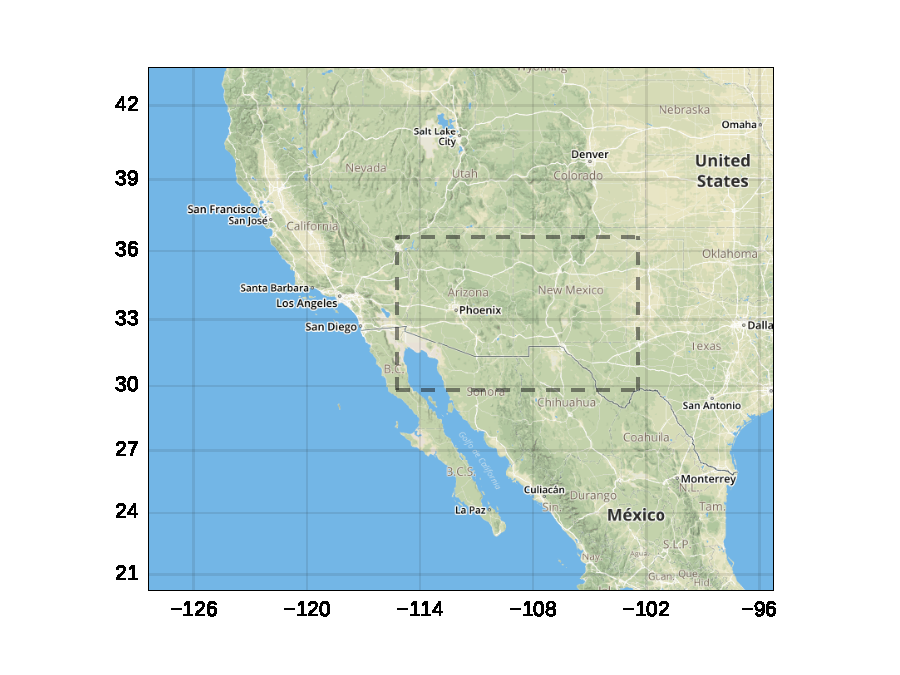
\includegraphics[width=0.9\textwidth]{figs/domains.pdf}
\vspace{-1.5em}
\caption{Outer and inner WRF domains}
\label{fig:wrfdomains}
\end{figure}

Each day, we produce six forecasts with WRF using the forecasts from
the North American Mesoscale Forecast System (NAM) and the Global
Forecast System (GFS).
The forecasts from the NAM and GFS at 00Z, 06Z, and 12Z each day serve
as the initialization and boundary conditions for the WRF forecasts for
a time-lagged ensemble.
Occasionally, extra WRF forecasts with initializations from the High
Resolution Rapid Refresh (HER'S) model are created primarily for
intra-day forecasts of severe weather.

With these six new WRF forecasts each day, along with some forecasts
from the previous day, we produce three irradiance forecasts.
One of these forecasts is a best estimate of the irradiance that is a
mean of the entire WRF ensemble.
We also produce minimum and maximum irradiance forecasts to provide a
confidence interval for the mean forecast.
As discussed in \cref{chap:future_work}, improved blending and WRF
ensemble techniques will be studied in the future.

One challenge with the WRF forecasts is the size of the forecast
files.
We produce files for surface parameters with three minute resolution
out to ten days in some cases at the 1.8 km horizontal spacing of the
inner domain.
These files may be as large as 47 GB in NetCDF4 classic format.
We found that accessing a single point forecast from these files could
take as long as ten minutes.

To overcome this slow access time, we first designed a system that
abstracts the access to the WRF files and then stores the point
forecasts in a Redis in-memory database for future access.
This system allowed us to access a point forecast in a few
milliseconds once it is initially loaded into Redis.
To reduce the tens of minutes that it takes to load the forecasts into
the Redis database the first time, we convert the files to NetCDF4
format with compression and rechunking.
Compression reduced the file size, and amount of data that may be read
from the disk, from 47 GB to 19 GB.
This rechunking greatly reduced point forecast access times because of
how the forecasts are stored on disk.
When the forecasts files are written by WRF, all gridpoints at one
forecast time are written in a single chunk.
By rearranging the chunks within a file so that they are chunked with
only a few gridpoints and all the forecast times, we
only need to read a few chunks of data from disk in order to get the
point forecasts we are interested in instead of the entire file.

With irradiance forecasts generated, we then need to convert from
irradiance to power.
To perform this conversion, we carefully analyze the
production data and produce clear-sky expectations for each power
plant.
Then, we convert irradiance forecasts into clear-sky index forecasts
and multiply by the clear-sky expectation for the power plant to
produce a power forecast.
This produces forecasts that are within a few percent of the actual
power produced on clear days.
In the future, improved modeling of the system directly incorporating
module and inverter parameters along with secondary variables such as
temperature will be studied.

\begin{figure}[htb]
\centering
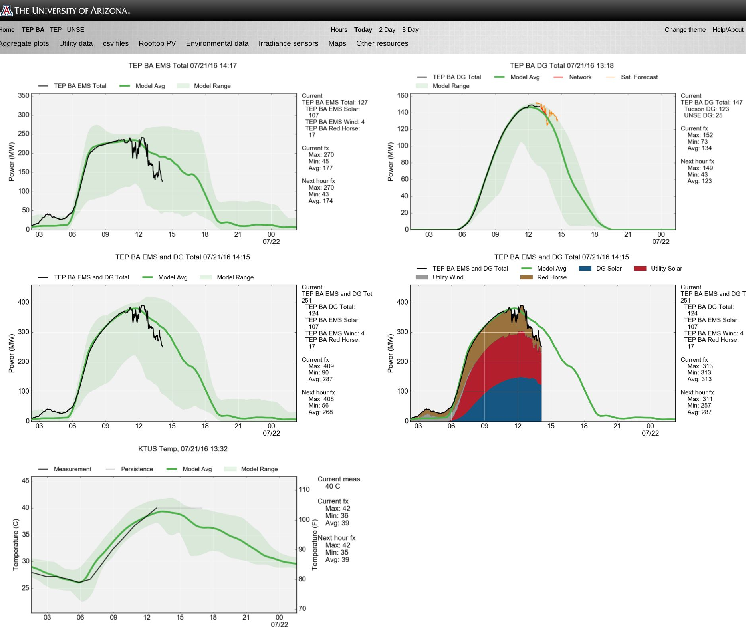
\includegraphics[width=0.8\textwidth]{figs/web_example.pdf}
\caption{Screenshot of the forecasting website}
\label{fig:website}
\end{figure}

The software that extracts the data from the WRF files, generates the
other forecasts, combines them together, converts the irradiance
forecasts to power forecast, and generates CSV files and plots of the
forecasts is currently a monolith written in Python.
The plots are then presented on a website that the utilities can
access as in \cref{fig:website}.
They can also download the CSV files with the forecast data from the site.
We also operate a public website with primarily forecasts of weather
variables (temperature, wind, etc) at
https://forecasting.energy.arizona.edu/public.
In addition to the website with the forecast graphics and CSV
downloads, we also have a REST API to programatically access the
forecast data.

\section{Future Improvements}
\label{sec:futurefx}

In addition to the new forecasting methodologies and techniques
discussed in \cref{chap:future_work}, we also plan to improve the
forecast generation software.
The current forecasting monolith has grown complex and difficult to
debug and it lacks sufficient test coverage.
Furthermore, the process consumes large amounts of memory and can take
up to five minutes to generate a new forecast and all the associated
figures.
A new framework will be more distributed with unit tests for nearly
every line of code.
It will be easier to incorporate new and developing
forecasting techniques into the framework, and new forecasts should be
generated in under a minute.
An overview of the new framework is shown in \cref{fig:nabu}.

\begin{figure}[htb]
\centering
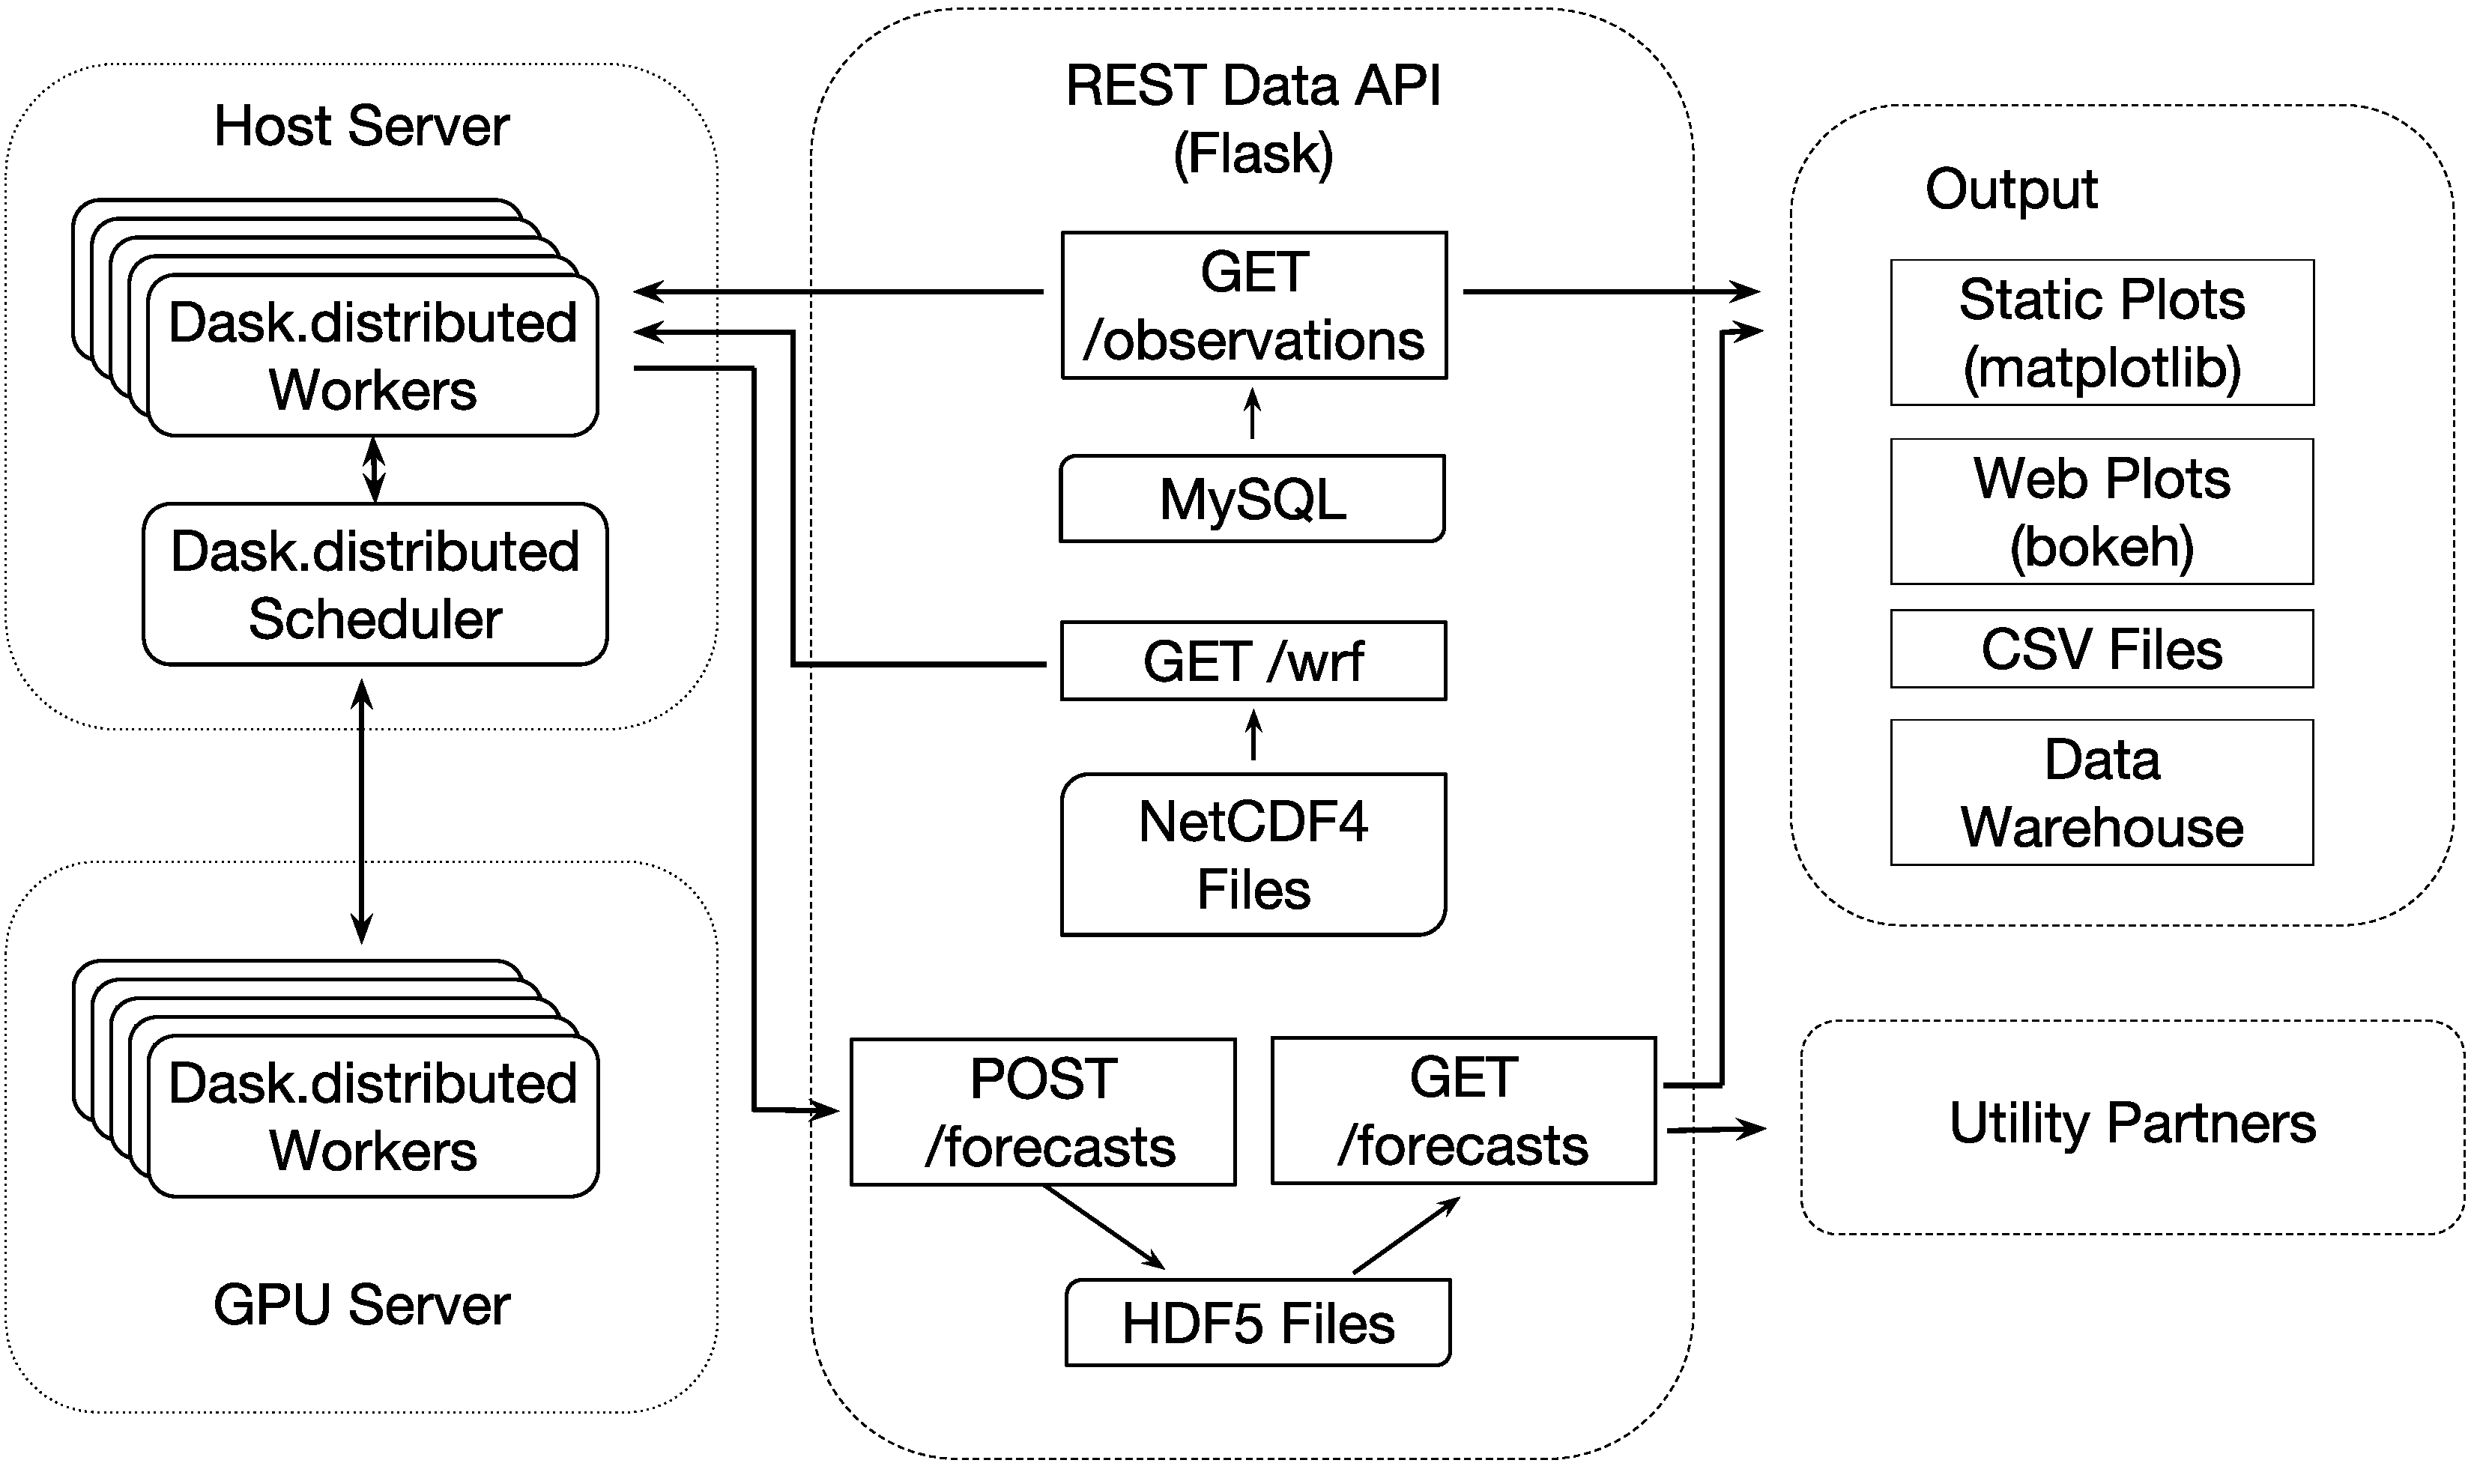
\includegraphics[width=0.9\textwidth]{figs/nabudiagram.pdf}
\caption[Diagram of the future forecasting system]{A diagram of the
future forecasting system. The WRF and measurement data is retrieved
from the API. Then, Dask workers generate the forecasts and upload
them to the API. The forecasts can then be retrieved from the API by
utility partners or by plot generators.}
\label{fig:nabu}
\end{figure}

The new framework relies on the Python library Dask.
With Dask, we first define a computation based on the inputs,
functions to execute, and outputs.
Dask then generates a computation graph and the computation can be
distributed to a number of worker processes that may reside on
multiple machines.
Dask also allows task to be distributed based on machine requirements
such as the presence a GPU to perform the satellite optimal interpolation.
The computation graph can be stored with each forecast along with
package version information to provide provenance of how the forecast
was generated for better reproducibility.

The second primary component of the framework is the data API.
This API will allow for any client with a connection to the API to
retrieve data from WRF files or MySQL with a simple GET command.
The API will also be responsible for storing the generated forecast
data in a proper format, and retrieving that data to send to the
utility companies or to other output processes.
The API will be built as a set of microservices so that components can
be upgraded individually.

The third component of the framework is the output layer.
Here, static plots, dynamic plots, and CSV files will be generated for
the current web portal.
This decoupling of the plotting and forecast generation should allow
for faster forecast generation times, and even faster plotting since
it will make it easier to distribute the plotting to multiple
processes.




%%% Local Variables:
%%% mode: latex
%%% TeX-master: "dissertation"
%%% End:
